\documentclass[12pt]{article}
\usepackage[english]{babel}
\usepackage{tikz}
\usepackage{graphicx}
\usetikzlibrary{decorations.pathmorphing} % noisy shapes
\usetikzlibrary{fit}		% fitting shapes to coordinates
\usetikzlibrary{backgrounds}	% drawing the background after the foreground


\title{Using Tweets and Bayesian Statistical Modeling to predict the 2012 Presidential Elections}		
\author{Hillary Sanders}	
\date{Nov 7 2012}				

\begin{document}
\maketitle				

\begin{abstract}
To determine the posterior probability that President Obama will win this year's 2012 Election, I created a forecasting model which predicts state-level vote-share probabilities by using a hierarchical Bayesian model to incorporate the simple text analysis of state-specific tweets into predictions. The model uses MCMC methods to develop the final posterior distribution. Model priors were based off of state-level 2004 and 2008 vote-share data. Data consisted of recent tweets mentioning `Obama' or `Romney'. Although the simple text analysis of tweets is not a perfect substitute for polling data (problems will be discussed below), it offers a potential way to bolster political forecasting models. The focus of this project, then, was not to predict the 2012 election with the great accuracy, but rather to be able to roughly gauge the potential effectiveness of simple tweet text analysis. 
\end{abstract}

\section{Introduction}
Social media analysis used as a means of prediction is a tantalizing, but very tough sell. It's difficult to train on, because social media users, social media patterns, and the world that social media is describing all change over time. If you don't use training data (this project doesn't), it's difficult to precisely determine how your raw input (e.g. tweets) corresponds to the thing you're predicting (e.g. votes). In my case, I treated tweets as poll votes. $\\$ $\\$
  Another difficult problem to be faced is the fact that social media users are generally not a random sample of the population you're predicting for. Twitterers surely do not represent the average American voter. $\\$ $\\$
  Still - the potentials of using social media to learn and predict things are vast. Take this paper's example of predicting elections. Even polls themselves do not take random samples of voters, but they still offer a high quality source of data. However, polls are expensive, and thus limited. But tweets are free, and the number of tweets to analyze is huge and growing. If social media could offer a substandard - but still beneficial - substitute for expensive and sparse sources of data (like polls), prediction models could be supplemented and improved upon by using social media as a proxy for polls. (Or, in some cases, social media analysis could even uncover trends that things like polls may not be able to, or uncover trends more quickly). 
  $\\$ $\\$
In this paper, I used the simple text analysis of tweets either mentioning 'Obama' or 'Romney' from all 50 states plus the District of Columbia to substitute for polling data (which substitutes for actual votes). I used these twitter 'votes' to modify each state's 2008 standardized vote-share to their predicted vote-share for this election. I used the OpinionFinder wordlist (Wilson, Wiebe, and Hoffmann 2005) - a list of words, either valued negatively or positively (-1, 1) - to conclude that each unique tweet is pro-Obama, pro-Romney, or neutral (to be thrown out). Neutral tweets either mentioned both candidates, or mentioned only one candidate but did not have more positive words than negative, or vice versa.  (For other options, see Brendan O�Connor et. al.)
$\\$ $\\$
Using MCMC methods (implemented with the R package rjags), I created a hierarchical Bayesian model to approximate the posterior probability that Obama will win each state, and from that, the posterior probability that Obama will win the 2012 presidential election. I found that because the simple text analysis of tweets that I used (seems to) so badly represents state-level vote-shares, my model is not to be trusted, and is fairly unstable. It predicts that Romney will win about 69\% of the time. Despite my model's failures, there is evidence that the simple text analysis of tweets is fairly strongly correlated with state-level historical vote-shares, and thus potentially useful.
$\\$
\section{Data}
The data I used were limited to the following: 
     \begin{enumerate} 
          \item State-level voting outcomes for the 2004 and 2008 presidential elections.
      \item Just over one million tweets taken from twitter's API using the R package twitteR, mentioning either Obama or Romney, and each specific to a state. Only about an eighth of these were judged to be both unique and non-neutral.
         \item The OpinionFinder wordlist - a list of about 1600 negative and 1200 positive words (Wilson, Wiebe, and Hoffmann 2005).
           \end{enumerate}
(1) was used for prior probabilities, and the estimation of prior hyper-parameters. (3) was used to create 0-1 polling-like data from (2). The 0-1 data was used to estimate the posterior probability of each state's vote-share, which was then used to estimate the posterior probability of Obama winning the election.

\section{Methodology: A Bayesian Forecasting Model}
In my model, a state $i$'s vote-share was modeled by treating tweets as 0-1 votes (0 for Romney, 1 for Obama). For each state $i$, the sum of this 0-1 tweet data was assumed to be a pull from a binomial distribution, with $p$ equal to the 2008 election vote-share in state $i$, plus some change factor. The change factor was distributed by a combination of normal and beta distributions. I estimated the hyper-parameters to this combined distribution by inspecting standardized state-level changes in vote-shares from  the 2004 and 2008 Presidential elections (pro-Democrat or pro-Republican trends were corrected for). Model checking favored this combination of distributions (see code).

\subsection{Specification}
For all $i$ in $1:51$ 'states' (includes DC), denote the following: $\\*$
Let $p_i$ represent the true probability that a voter from state $i$ will vote for Obama. Let $\phi_i$ represent state $i$'s Democrat vote-share in 2008. Let $\theta_i$ represent $p_i$ - $\phi_i$. Then $p_i$ = $\theta_i$ + $\phi_i$, and $\hat p_i$  represents the predicted probability that a voter from state $i$ will vote for Obama. $\\$ $\\$
For each state $i$, let $t_i$ represent the scraped set of non-neutral tweets from state $i$'s tweets. Then for each element in $t_i$, there is a 0-1 element $j$ in $x_{i}$, representing whether state $i$'s $j$th tweet was judged to be be a pro-democrat or pro-republican tweet. Then the sum of all elements in $x_{i}$ is assumed to be a pull from a binomial($p_i$) distribution, where n is equal to the length of $x_i$ (i.e. the number of non-neutral, unique tweets from state $i$).


\begin{figure}
\centering
% The state vector is represented by a blue circle.
% "minimum size" makes sure all circles have the same size
% independently of their contents.
\tikzstyle{blue}=[circle,
                                    thick,
                                    minimum size=1.2cm,
                                    draw=blue!80,
                                    fill=blue!20]

% The measurement vector is represented by an orange circle.
\tikzstyle{yellow}=[circle,
                                                thick,
                                                minimum size=1.2cm,
                                                draw=orange!80,
                                                fill=orange!25]

% The control input vector is represented by a purple circle.
\tikzstyle{red}=[circle,
                                    thick,
                                    minimum size=1.2cm,
                                    draw=purple!80,
                                    fill=purple!20]

% The input, state transition, and measurement matrices
% are represented by gray squares.
% They have a smaller minimal size for aesthetic reasons.
\tikzstyle{matrx}=[rectangle,
                                    thick,
                                    minimum size=2cm,
                                    draw=gray!80,
                                    fill=gray!20,
                                    ]

\tikzstyle{whitespace}=[rectangle,
                                    thick,
                                    minimum size=1.1cm,
                                    draw=white!80,
                                    fill=white!20,
                                    ]


\begin{tikzpicture}[>=latex,text height=1.5ex,text depth=0.25ex]
    % "text height" and "text depth" are required to vertically
    % align the labels with and without indices.
  
  % The various elements are conveniently placed using a matrix:
  \matrix[row sep=0.25cm,column sep=.25cm] {
    % First line
    &
        \node (normal-1) [red]{$\alpha$ Normal}; &
        &
        \node (normal-2)   [red]{$\beta$ Normal};     &
        &
        \node (normal-3) [red]{$\sigma^2$  Gamma}; &
        \\
        \\

        % Second line
        % HACK HACK HACK. Neh how to move stuff? ...
        \node (whitespace)   [whitespace] {};       &
        \node (whitespace)   [whitespace] {};       &
        \node (whitespace)   [whitespace] {};       &
        \node (abs)   [matrx] {$\alpha$, $\beta$; $\sigma^2$};       &
        \\
        \\
        % Third line
        \node (whitespace)   [whitespace] {};       &
        \node (th1) [blue] {$\mathbf{\theta}_{1}$}; &
        \node (A_k-2)         {$\cdots$};           &
        \node (th2)   [blue] {$\mathbf{\theta}_i$};     &
         \node (A_k-2)         {$\cdots$};           &
        \node (th3) [blue] {$\mathbf{\theta}_{n}$}; &

        \\
        % fourth line
        &
        \node (x1) [yellow] {$\mathbf{X}_{1}$}; &
          \node (A_k-2)         {$\cdots$};           &
        \node (x2)   [yellow] {$\mathbf{X}_i$};     &
          \node (A_k-2)         {$\cdots$};           &
        \node (x3) [yellow] {$\mathbf{X}_{n}$}; &
        \\
    };
    
    % The diagram elements are now connected through arrows:
    \path[->]

        (normal-1) edge (abs)
        (normal-2) edge (abs)
        (normal-3) edge (abs)
        
        (abs) edge (th1)			
        (abs) edge (th2)
        (abs) edge (th3)

        (th1) edge (x1)
        (th2) edge (x2)
        (th3) edge (x3)
        ;
 
\end{tikzpicture}

\caption{Directed Acyclic Graph of my Hierarchical Bayesian Model}
\end{figure}


\subsection{Model}
My model tries to predict $p$, and $\phi$ (2008 vote-shares) is already known, so all that is needed is to decide on a distribution for $\theta$. After significant model checking, it was clear to me that $\theta$ is quite unlikely to be normal, t-distributed, or beta. The distribution should be symmetric and centered around zero, though, so choices were limited. $\\$ 

 An equal combination of a beta distribution (centered around .5, and then subtracted from by .5) and a normal distribution (centered around zero) actually fit the difference in state-level vote-shares from 2004 to 2008 quite well, meaning that that combination was a good distribution to assume for $\theta$.  
 $\\$ $\\$
 The parameters on this normal-beta distribution, and the weighting of each can be estimated, but are not certain things. For this reason, I put normally distributed priors on $\alpha$ and $\beta$, and a gamma (non-zero) prior on $\sigma^2$. There are 'best guesses' for $\alpha$, $\beta$, and $\sigma^2$ (for details, see code), so unimodal distributions made sense, but there is still uncertainty. On average, the resultant prior beta distribution had a standard deviation of about .04, and the resultant prior normal distribution had a standard deviation of about .05. These values were most consistent with standardized state-level differences between the 2004 and 2008 vote-shares. The  standard deviation of these priors were (somewhat arbitrarily) estimated from the data. $\\$ $\\$ 
 I also placed a uniform(.2,.8) prior on the weighting of the normal and beta part of the $\theta$ distribution. 
 $\\$
\includegraphics[scale=.6]{prior2.pdf}
$\\$
Above, you can see 1000 simulations of $\theta$ plotted with the standardized (mean=0) differences between state-level vote-shares from the 2004 and 2008 elections. Below, you can see that various model checking tests passed. (The red lines represent the observed, standardized, 2004-2008 value, while the histograms represent simulations.)
 
\includegraphics[scale=.4]{priormax.pdf}
\includegraphics[scale=.4]{priormin.pdf}
\includegraphics[scale=.4]{prorsd.pdf}


\subsection{Model Convergence and Posterior Prior Probabilities}
From the two graphs below, it seems that the model did converge, although some variables tended to bounce around a lot.
$\\$ $\\$
\includegraphics[scale=.6]{trace1.pdf} $\\$
Above, $alpha$, $beta$, and $precision$ refer to the two distributions (beta for alpha and beta, normal for precision) that make the $\theta$ distribution. Below, $nbweight$ is the weight of the normal to beta distributions (added together to make the $\theta$ distribution), and $p_1$ is the predicted p value for state 1 (Alaska). Trace plots of the other $p_i$'s look similar.
$\\$
\includegraphics[scale=.6]{trace2.pdf}
$\\$ $\\$
Because tweet-votes were such bad estimates of actual votes (or so it seems, looking at historical state-wide vote-shares) the posterior probabilities of $p$ were very often much larger than original priors suggested. Original priors of alpha, beta, and sigma predicted a standard deviation in $\theta$ of about 4\%, with quite small resultant standard deviations on this standard deviation prediction. But because of the thousands of tweets that often argued to the contrary for each state, these priors were made nearly insignificant. (Note that this is in part due to the construction of the model, and because tweets were treated specifically as real votes pulled from the real population of voters, so it could be easier to see the effect of using tweets for prediction - in a regular prediction model, this would not be the case.)

\section{Results}
In terms of who will win the 2012 Presidential Election, my model predicted that Mitt Romney will win - about 69\% of the time (see graph below). But guessing  who will win the election was not the main goal of this project. In fact, there is good evidence that this is a distinctly bad model, whose predictions should not be trusted.  $\\$
\includegraphics[scale=.55]{winner.pdf}  $\\$
 Below, standardized 2008 state-level vote-share values (rainbow) were plotted with my model's posterior 90\% confidence intervals, along with each state's tweet-share (smaller black dots). Standardized 2008 vote-share values often fell far from my model's posterior 90\% confidence intervals. Basically, tweet-shares were so different from vote-shares, that the tweet-shares overpowered their relatively snug priors, resulting in confidence intervals that often didn't include historical vote-shares. (Note that standardized 2008 vote-shares $are$ the maximum likelihood estimates from the model with no tweet data.) All states highlighted with a pink line had 2008 vote-share values that fell within the model's 90\% confidence interval.
$\\$  $\\$
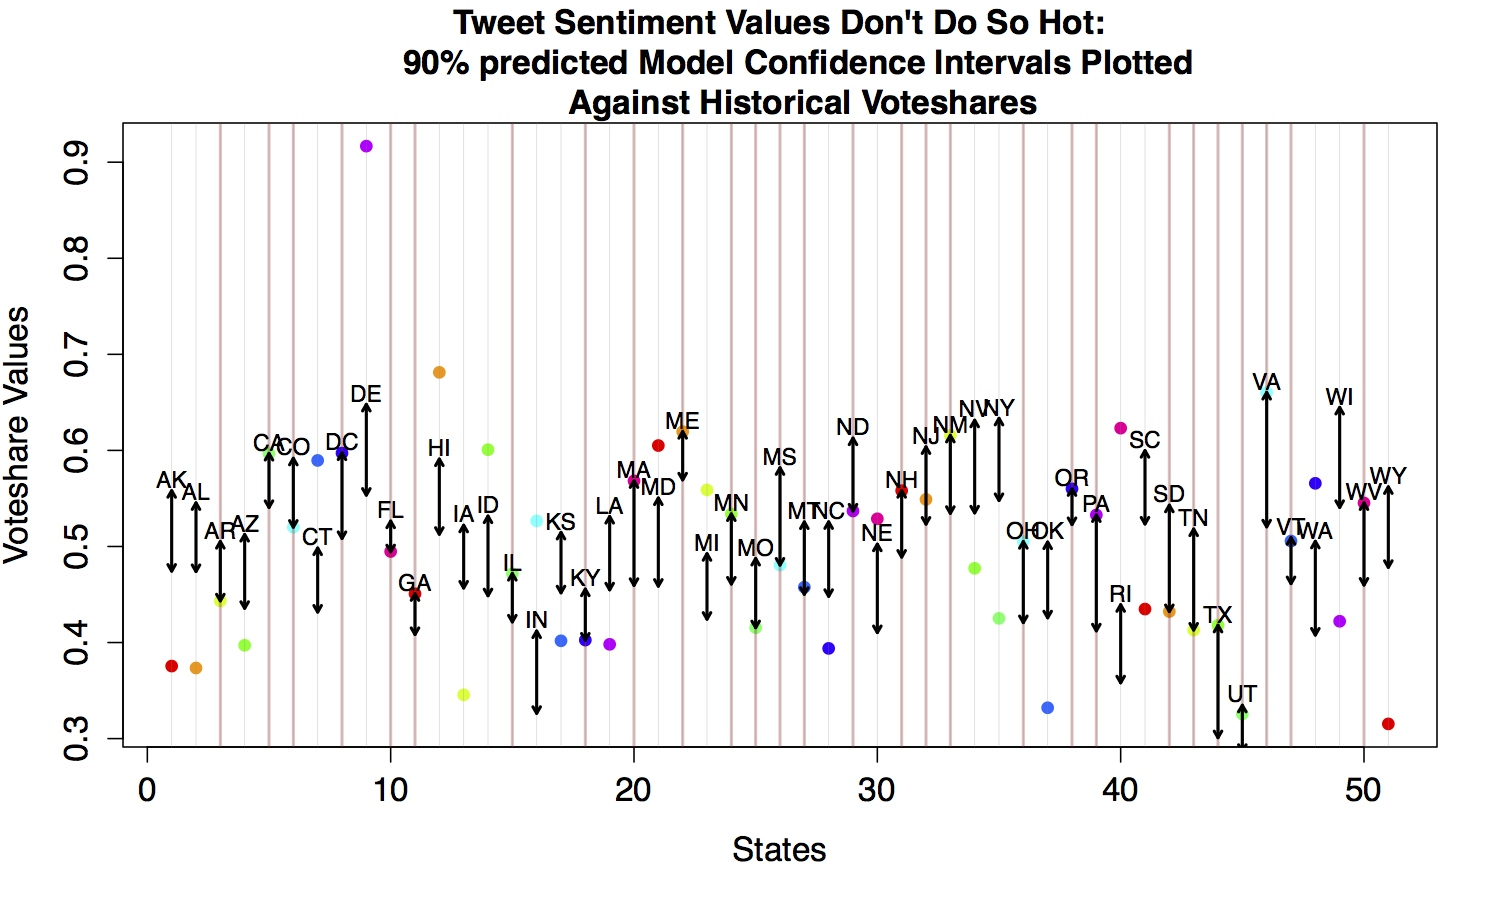
\includegraphics[scale=.6]{rainbow.pdf}
$\\$
 Making the priors tighter would fix this, to a certain extent, but the goal of my model was to investigate the effectiveness of tweets as election predictors, as opposed to just predicting the 2012 presidential election with 2008 values. Still, it's interesting to see the effect. A modified distribution of $\theta$ produces a similar graph, which you can see below. (Note that this particular graph does $not$ correspond to the rest of the paper, analysis, outcomes, and assumptions!) Here, every single state's historical value falls within the model's 90\% confidence interval, while the model predictions still manage to deviate significantly from historical values.
 $\\$ $\\$
 \includegraphics[scale=.65]{rainbow2.pdf}
$\\$
The main point of this project was to roughly evaluate the potential effectiveness of tweets in political prediction models. And these 'effectiveness' results of my model suggest that such a crude and basic analysis of tweets is not a fantastic way to predict elections. Tweet-shares (the way I calculated them) trend towards 50/50 pro-democrat pro-republican, whereas actual state vote-shares are likely to be much less even. You can see this in the figure below, where each state's tweet-share is plotted as a node, size corresponding to the number of tweets used to calculate its tweet-share, with an arrow connecting each state's tweet-share node to a smaller black node representing its 2008 vote-share. Historic values are generally pulled towards the 50\% mark to meet their state's tweet-share value. 
$\\$ 
\includegraphics[scale=.63]{purple.pdf}
 $\\$
Even when this disparity in standard deviation from 50\% is corrected for by transforming tweet-shares, tweet-shares and historical vote-shares do not match as much as we would like them to. In short, there is a correlation between tweet-shares and historical vote-shares, but it is relatively weak, showing that tweet-shares alone are not a good way to predict future elections, and would be more useful if they were not treated as representative, random samples of votes.
$\\$ $\\$ 
 My results suggest that either I caught too much noise (my text analysis is too simple), or tweets aren't very representative of the average voter. Still, there is a chance that simple tweet text analyses may catch something that polls so not. If you could know that the twitter population represents some defined set of the voting population, then twitter could be used to replace or supplement predictions for that defined set of the voting population, leaving polls to predict for everyone else. It could even be that tweet analyses correlate quite well to that small marginal shift from other forecast's predictions to the current election's vote-share values... But, I can't test that hypothesis until after I turn in this midterm for dreaded grading.
$\\$ $\\$
\includegraphics[scale=.65]{hope.pdf}
\includegraphics[scale=.65]{regression.pdf}


\section{Conclusion}
Although this model - as a model - is more or less a bust, there does seem to be a significant and positive relationship between tweet sentiment scores regarding a political candidate, and past vote-shares. So it is quite conceivable that better models could actually use tweets as a proxy for polls, or even as a means to uncover trends and underlying structures in voting tendencies that polls cannot acquire, or uncover trends more quickly and cheaply than polls otherwise could acquire. 

\newpage

\section{Bibliography}
Wilson, T.; Wiebe, J.; and Hoffmann, P. 2005. Recognizing contextual polarity in phrase-level sentiment analysis. In
Proceedings of the Conference on Human Language Technology and Empirical Methods in Natural Language Processing
$\\$ $\\$
Brendan O�Connor et. al. 2010. From Tweets to Polls: Linking Text Sentiment to Public Opinion Time Series. In Proceedings of the Fourth International AAAI Conference on Weblogs and Social Media

$\\$ $\\$ $\\$
$\\$ $\\$ $\\$
$\\$ $\\$ $\\$
$\\$ $\\$ $\\$
$\\$ $\\$ $\\$ 
$\\$ 

\includegraphics[scale=.4]{twitter.png}
\includegraphics[scale=.4]{twitter.png}
\includegraphics[scale=.4]{twitter.png}


\end{document}          








  